\section{Triplanar-Net}
\label{chapter5}

It is computationally demanding to work with three-dimensional volumetric data, and consequently with three-dimensional neural networks (such as the ones shown in chapter \ref{chapter4}); this applies even more so for the case of aneurysm segmentation where localization is difficult due to the size of aneurysms. This could be overcome by using low-resolution data or by using shallow networks, however this would adversely affect performance. Therefore the proposed network architecture works with 2D projections of patches of the volumetric data. Since we are working with cerebral TOF-MRAs for the task of aneurysm segmentation, the projections used are axial, coronal and sagittal Maximum Intensity Projections (MIPs). 

To obtain better 3D context, 3D reconstruction using the orthogonal views is carried out within the network and the network is trained on 3D labels. This removes the need to naively reconstruct the label after obtaining 2D labels, and also allows the network to learn 3D context while still being lightweight and non-resource intensive. 

The input arms (and concept of using 2D MIPs) is heavily inspired by the BtrflyNet architecture, but the input portion is made deeper and an added axial view is also used \cite{sekuboyina2018}. During inference, the sagittal and coronal output heatmaps of the BtrflyNet architecture are combined using the outer product to create a 3D heatmap. Triplanar-Net similarly uses the outer product to reconstruct a 3D volume, although this is done within the network architecture and 3D labels are also used for training the network unlike for the BtrflyNet architecture.


\subsection{Maximum Intensity Projection}
Maximum Intensity Projection is a method that consists of projecting the voxel with the highest intensity lying in the direction of the plane of projection. It allows representing three-dimensional objects in two dimensions. MIPs have several advantages: vascular structures are well defined and appear clearly as tubular branching structures, the susceptibility to noise is highly reduced due to projecting only the maximum value across a view, and through MIP the use of two dimensional images immensely reduces required resources and parameters. Figure \ref{fig:mip} shows axial, coronal and sagittal MIPs obtained from two positive cases in the dataset. 

\begin{figure}[h]
	\centering
	\begin{subfigure}{\linewidth}
		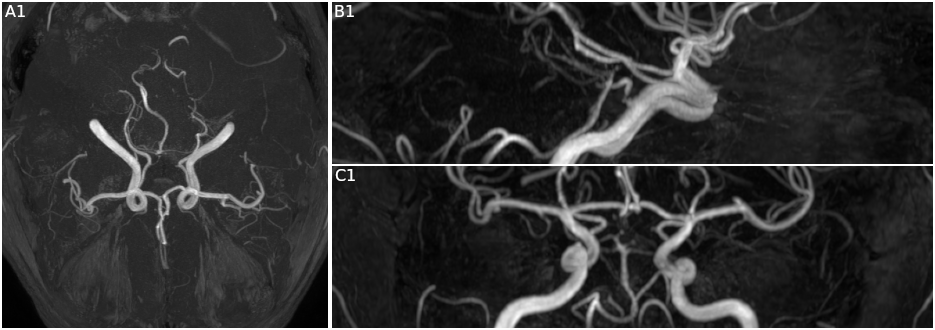
\includegraphics[width=\linewidth]{figures/mip_10021.png}
%		\phantomsubcaption
%		\label{fig:mip_10021.png}
	\end{subfigure}
	\begin{subfigure}{\linewidth}
		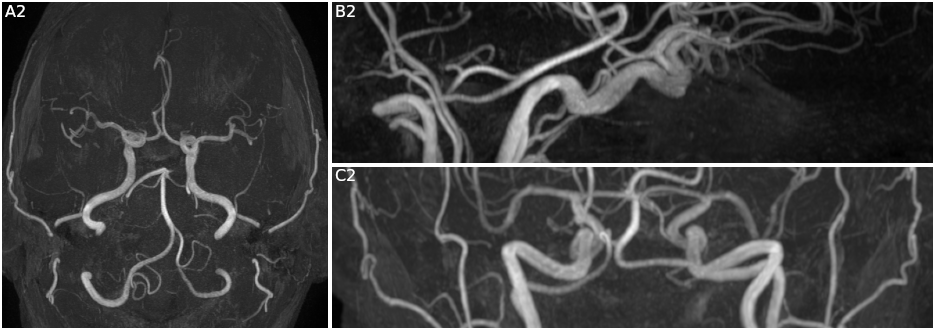
\includegraphics[width=\linewidth]{figures/mip_10028.png}
%		\phantomsubcaption
%		\label{fig:mip_10028.png}
	\end{subfigure}
	\caption[Maximum Intensity Projections of two positive cases.]{Images A1 and A2 show axial MIPs of two different cases that contain UIAs, and similarly B1, B2 and C1, C2 show sagittal and coronal views of MIPs respectively. The cases used are from the train dataset available via the ADAM challenge \cite{Timmins2020}.}
	\label{fig:mip}
\end{figure}

\begin{figure}[t]
	\centering
	\begin{subfigure}{\linewidth}
		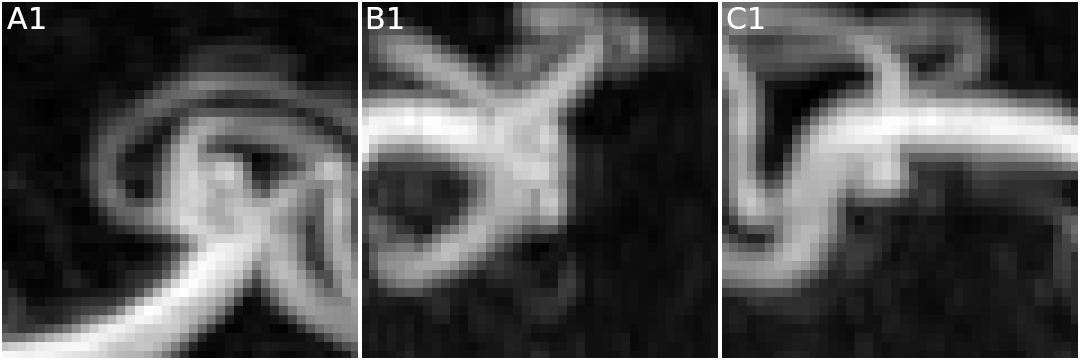
\includegraphics[width=\linewidth]{figures/mip_patch10021.png}
	\end{subfigure}
	\begin{subfigure}{\linewidth}
		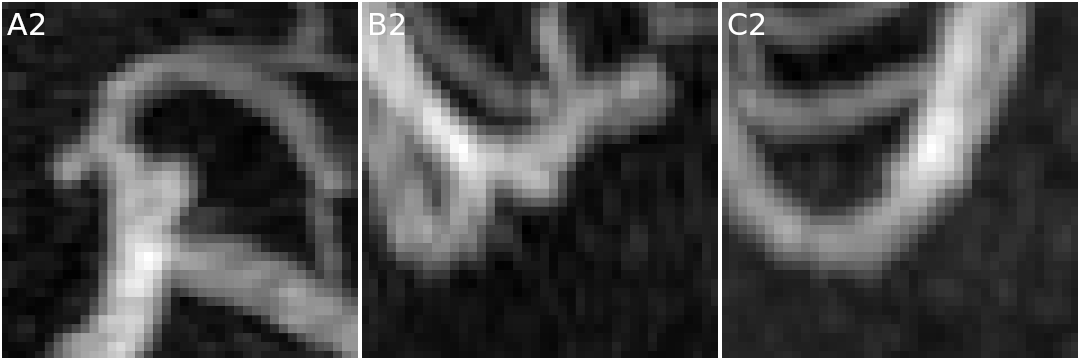
\includegraphics[width=\linewidth]{figures/mip_patch10028.png}
	\end{subfigure}
	\caption[Patches of Maximum Intensity Projections of two positive cases.]{Similarly to Figure \ref{fig:mip}, patches of axial, sagittal and coronal (A, B, and C) MIP images of two positives cases, are shown -- with the 3D patch from which the MIP is taken extracted with the aneurysm centered.}
	\label{fig:mip_patch}
\end{figure}


As discussed in chapter \ref{chapter3}, the size of aneurysms in a TOF-MRA is very small; the mean diameter of an aneurysm in our dataset being $4.11$ mm. With a re-sampled volume with voxel spacing $0.3 \times 0.3 \times 0.3$ mm\textsuperscript{3}, the mean shape of a volume encompassing an aneurysm would be $21.5 \times 21.5 \times 21.5$ -- assuming a spherical structure of the aneurysm. Axial, coronal and sagittal images (after preprocessing of the TOF-MRA volumes) would have shapes $512 \times 512$, $512 \times 140$, and $512 \times 140$ respectively. Due to this, an MIP taken of the whole three-dimensional TOF-MRA volume, would have little useful information regarding the aneurysm, such as an enlarged vessel. Therefore, as most other training procedures for other networks, Triplanar-Net is trained using patches of the whole volume. MIPs are then taken for the patch of cropped volume, further allowing the network to learn important features with respect to the aneurysm segmentation such as structure and shape. The projections the network learns from are thus as in Figure \ref{fig:mip_patch}, which are obtained from sampling a TOF-MRA volume. There are other projection methods, however using MIP for cerebral TOF-MRA is appropriate for this task due to the focus on vessels. 

\subsection{Network architecture}
The proposed Triplanar-Net is a CNN producing a binary segmentation the same size as the 3D patch used to create the MIPs. The model consists of an axial, coronal and sagittal 2D encoder path, a 2D to 3D reconstruction block, and a 3D decoder path, along with skip connections -- see the full architecture in Figure \ref{fig:trinet.pdf}. 

\img{trinet.pdf}{\linewidth}{Proposed network architecture for Triplanar-Net. Three input arms each take an MIP of either the axial, coronal or sagittal view extracted from a 3D patch. The inputs are encoded using 2D convolutions operations and max pooling before going through the 2D to 3D reconstruction block, and being decoded with 3D transpose convolutions followed by 3D convolutions. The convolution kernel size, padding size, and stride are represented as \{kernel.padding.stride\} in the image and the number of channels is shown within each block.}{Triplanar-Net architecture.}

\img{2d_to_3d.pdf}{0.5\linewidth}{Diagram of the 2D to 3D reconstruction block used in the Triplanar-Net architecture. Three inputs are given to the block -- representing the axial, sagittal and coronal MIPs. A 2D convolution with a kernel size of 3, padding 1 and stride 1 is applied to each input. The orthogonal views are then combined by taking the outer product, and a 3D convolution with kernel size of 3, padding 1 and stride 1 is applied to reconstructed 3D image.}{2D to 3D reconstruction block.}

In each encoder path a $1 \times 1$ convolution is applied to the respective input MIP, after which follow three layers containing $3 \times 3$ convolutions (with stride of 1 and padding 1) plus max-pooling with a stride of 2. 
In the the 2D to 3D reconstruction block, a convolution with kernel size $3 \times 3$ is applied to each of the feature maps of the axial, coronal and sagittal encoder paths. The 3D downsampled representation is constructed by calculating the outer product of the feature maps from the three orthogonal views, and applying a $3 \times 3 \times 3$ convolution. Figure \ref{fig:2d_to_3d.pdf} shows the 2D to 3D reconstruction block.
Lastly, to upsample the reconstructed 3D representation, the decoder path applies three layers of $4 \times 4 \times 4$ transpose convolutions (stride 2 and padding 1) followed by $3 \times 3 \times 3$ convolutions (stride 1 and padding 1). To take advantage of higher resolution features, skip connections are added that concatenate the output of each convolution operation in the encoder path to an equivalent decoder operation. As the decoder path incorporates three dimensional representations, the high-res features are also passed through their own 2D to 3D reconstruction block. The 3D binary voxelized segmentation of the aneurysm is obtained after applying a $1 \times 1 \times 1$ convolution. To introduce non-linearities to the model, each convolution operation (2D, 3D, and 3D transpose) with a kernel size greater than 1 is followed by an ELU activation function. Batch normalization is also applied after convolution operations (2D, and 3D) in the encoder and decoder paths.

Unlike the BtrflyNet architecture, Triplanar-Net constructs a 3D representation within the model (prior to the decoder path) and also does not contain a middle arm that concatenates the feature maps of the three encoder paths. Using a 3D decoder path allows the model to learn valuable 3D context when upsampling the naively reconstructed 3D feature maps, which would otherwise be lost if only 2D feature maps were involved. The parameters in the decoder path also allow to obtain a much more detailed binary segmentation, compared to that of a 2D decoder -- i.e. there would be a lot of aliasing when reconstructing a 3D output from three orthogonal MIP binary outputs for example, therefore it is more effective to create a reconstructed intermediate representation of the three projections within the network and obtain a 3D binary segmentation after decoding. 

As stated previously the axial, coronal and sagittal images used for training the network are obtained by finding the MIP in each view of a 3D patch cropped from the whole TOF-MRA volume. Multiple sampling schemes for extracting segments were tested; ultimately it was most successful to construct a training batch by extracting segments of size $32 \times 32 \times 32$ in which $90\%$ of the input samples correspond to background class and $10\%$ to foreground class (i.e. voxels containing an aneurysm). For cases in which there are no aneurysms in the TOF-MRA, all segments will only contain background class. This training strategy was employed as it reflects the most realistic distribution of foreground to background class within the data. The network is trained using dice loss which takes the form: 

\[L = 1 - \frac{2\sum_{i}^{N}p_{i}g_{i}}{\sum_{i}^{N}p_{i}^{2} + \sum_{i}^{N}g_{i}^{2}} \]

where $p_{i}$ and $g_{i}$ represent the voxel values of the predicted binary segmentation and the ground truth binary volume, summed over $N$ voxels \cite{milletari2016v}. The network is trained with 5-fold cross validation using the AdamW optimizer for 100 epochs per fold. L2 regularization of $1e-5$ is also used during training to reduce overfitting.

In comparison to the networks described in Chapter \ref{chapter4}, Triplanar-Net consists of a more shallow architecture, as well as both 2D and 3D convolutions. Generally, a shallower network can lead to poorer overall results be it for any task. However, by efficiently combining two dimensional and three dimensional data and convolutions, the network is able to be lightweight while being able to also accurately segment aneurysms from parent vessels.

Once trained, inference for a given input TOF-MRA volume proceeds as: segments of the volume are sampled on a grid, axial, coronal and sagittal MIPs are obtained for each segment and fed to the network. The output segmentation of the TOF-MRA volume is built by concatenating the network output of each segment.

The design for Triplanar-Net had been through many iterations after coming to the architecture shown in Figure \ref{fig:trinet.pdf}, the ablation study for the other tested designs is in Appendix \ref{appendix1}. Another method that was an interesting approach was to consider the segmentation of aneurysms as a 2-staged approach; in the first stage a patch of the whole 3D TOF-MRA volume is classified (i.e. aneurysm or no aneurysm) using a classifier network, and if a positive classification is given the aneurysm within the patch s segmented with the segmentator network (Triplanar-Net). This approach was also trained but the sensitivity and specificity achieved with the classifier network did not warrant using the 2-staged approach. Some results of this 2-staged approach can be seen in Appendix \ref{appendix1}.

%\todo{removed classifier/full pipeline part because think i can get it to work without}
%Training the network on only segments centered on the foreground (apart from negative cases) causes the network to produce segmentations with a high number of false-positives. To mitigate this as well as to allow Triplanar-Net to focus on accurate segmentation of aneurysms, it is proposed to add an initial classification step during inference on a TOF-MRA volume. The classifier evaluates whether a certain patch of the TOF-MRA volume contains a vessel with an aneurysm. If positively classified, the segment goes through to Triplanar-Net for aneurysm segmentation, and if negatively classified then no foreground pixels are segmented in the patch. The full framework for inference for any TOF-MRA volume can be seen in Figure \ref{full_pipeline.pdf}. The classifier network can also be seen in figure \todo{network for classifier}. The classifier network is trained on 3D segments of the same size as those used for training Triplanar-Net, using a uniform sampling scheme. We require that this classifier has a high sensitivity, and favors false-positives over false-negatives. Thus, it is trained using cross-entropy loss with a larger weight given to a positively classified volume. \info{elaborate/maybe write better}.
%
%\img{full_pipeline.pdf}{\linewidth}{\todo{caption}}{Full pipeline for inference.}
%
%Adding this classifier prior to Triplanar-Net is hypothesized to not heavily increase resource usage or heavily impede inference; most segments of the TOF-MRA volume will only go through one network (either the classifier or Triplanar-Net) since a very small number of segments (out of $N$ segments sampled from the TOF-MRA volume) contain an aneurysm. A segment is only processed by both the classifier and Triplanar-Net if an aneurysm is detected to be within it. The complete binary segmentation map for the TOF-MRA volume is then reconstructed by combining -- according to the coordinates of the sampled segment -- the $x$ binary segmentations from Triplanar-Net and $y$ binary segmentations that are known to not contain an aneurysm.
%
%An alternative to using this framework with a combined classifier and Triplanar-Net would be to use post-processing after obtaining the binary segmentation map of a segment and altogether not use the classifier at all. However, this was opted against as this \todo{Why not?}
%
%\todo{ablation study in appendix to show design choices, i.e. no skip blocks, no combination path, 2d decoders instead of 3d}




